\section{High Performance Computing}
Con \textit{High Performance Computing} (\textit{HPC}) si intende l'utilizzo di multiprocessori o cluster per effettuare computazioni concorrenti tale che porti a throughput ed efficienza elevati.

Hardware e Software devono essere strettamente collegati per permettere l'utilizzo massivo della parallelizzazione

\subsection{Parallelismo}
Esistono due tipi principali di parallelismo:
\begin{sitemize}
    \item \textbf{Parallelismo delle task} Quando diverse task possono essere esguiti indipendentemente, in questo caso possonoe essere facilmente allocate su diversi core.
    \item \textbf{Parallelismo dei dati} Quando si può operare indipendentemente su porzioni distinte dei dati, in modo da poter suddividere le porzioni su più core.
\end{sitemize}

\subsection{Utilizzo delle GPU}
Mentre per le CPU l'incapacità di aumentare la frequenza e lo spostamento verso sistemi sempre più parallelizzati ha portato ad una riduzione del miglioramento delle performance, le \textbf{GPU}, nate con l'obiettivo di \textbf{elaborare processi parallelamente} hanno continuato a seguire quanto ipotizzato da Moore.

\spacer
Grazie all'architettura \textit{CUDA} le schede video NVIDIA hanno reso possibile la semplice scrittura di programmi altamente paralleli.

Ad oggi si utilizzano CPU solo quando non si può ottenere una grande parallelizzazione, mentre GPU quando è possibile distribuire il carico su un enorme numero di core relativamente poco potenti.

\spacer
Alcune computazioni possono benificiare da un approccio misto tra CPU e GPU, in questo caso il trasferimento dei dati da una memoria all'altra può causare dei rallentamenti anche importanti.

Per questo è in alcuni casi conveniente utilizzare una \textbf{memoria condivisa} così da eliminare questo overhead.

Un'implementazione della memoria condivisa si vede nei chip Apple Silicon che presentano un'unica pool di memoria da cui CPU e GPU attingono.

\begin{figure}[H]
    \centering
    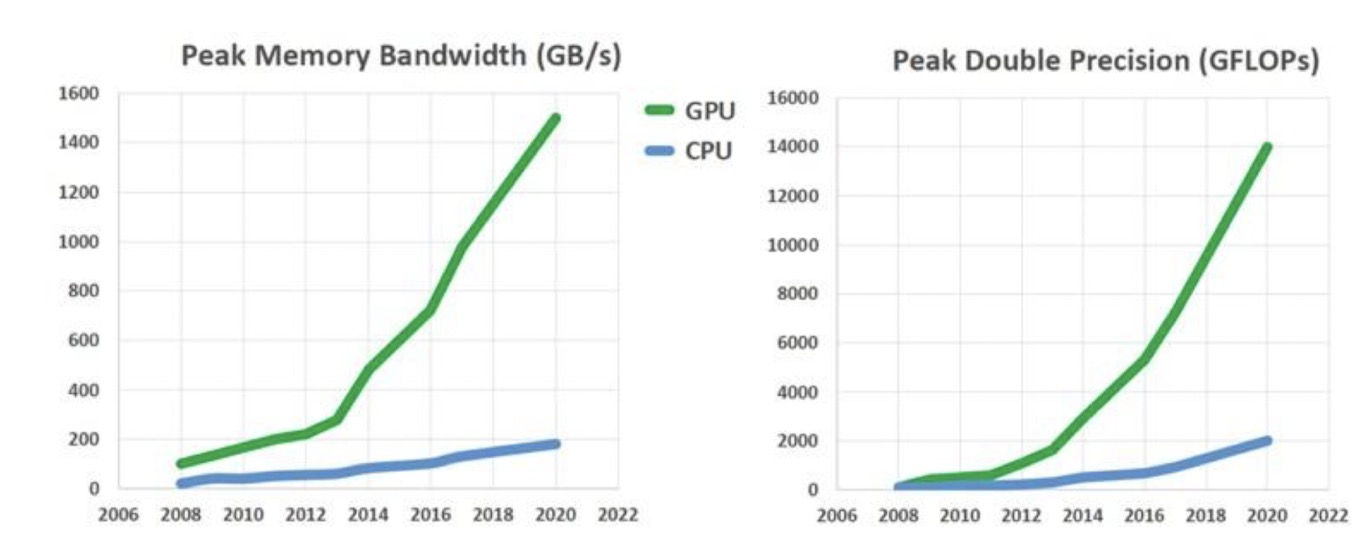
\includegraphics[width=0.65\linewidth]{assets/gflops-gpu-cpu.jpg}
    \caption{Gflops di CPUs e GPUs nel tempo}
\end{figure}

\subsection{TPU}
Da qualche anno Google si è dedicata allo sviluppo di una nuova tipologia di chip chiamati \textit{Tensor Processing Unit}, i quali hanno un set di operazioni ancora più ridotto rispetto alle GPU, ogni core ha quindi una superficie minore, rendendo così possibile stiparne un numero maggiore sullo stesso chip.

\spacer
Questi processori sono indirizzati al \textbf{Machine Learning}, in particolare all'esecuzione di algoritmi per l'allenamento di reti neurali

\subsection{FPGA}

I \textit{Field Programmable Gate Array} sono dei dispositivi che contengono dei blocchi logici configurabili, essi consentono di programmare dell'hardware per fornirgli particolari funzionalità.

\spacer
Essi permettono di implementare funzioni in hardware, con tutti i benfici che questo porta, senza dover sostenere i costi di fabbricazione di un chip.
